\documentclass{template/template}

%\renewcommand{\familydefault}{\sfdefault} %% Only if the base font of the document is to be sans serif
%\usepackage{bera}

\usepackage[T1]{fontenc} % evropské uvozovky
\usepackage{subcaption}
\usepackage{amsmath}
\usepackage{enumitem}
\usepackage{hyperref}
\usepackage{gensymb} % balíček symbolů
\usepackage{booktabs}
%\usepackage{lmodern}
\usepackage{csquotes} % text lze uvést do uvozovek pomocí \enquote{text}
\usepackage{textcomp}

\usepackage[toc,page]{appendix}
\usepackage{color} % balíček pro obarvování textů
\usepackage{xcolor}  % zapne možnost používání barev, mj. pro \definecolor
\definecolor{mygreen}{RGB}{0,153,153} % nastavení barev odkazů 
\definecolor{myblue}{RGB}{0,0,200} 
\definecolor{commentgreen}{RGB}{0,100,0} % nastavení barev pro příklady z C++
\definecolor{deepblue}{rgb}{0,0,0.7}
\definecolor{deepred}{rgb}{0.6,0,0}
\definecolor{deepgreen}{rgb}{0,0.5,0}
\usepackage{listings} % balíček pro formátování zdrojových kódů 
\usepackage[author=,status=draft]{fixme} % vkládání poznámek  
% dva módy (status): draft (poznámky se zobrazují v PDF) / final (poznámky se nezobrazují v PDF)
\usepackage{graphicx}
\usepackage{multirow}
\usepackage{float}


\usepackage[T1]{fontenc} % import tučného písma typu tt pro prostředí listings
%\usepackage{listings} % balíček pro obarvování syntaxe ukázek programů v textu
\usepackage{listingsutf8} %nutné pro \usepackage{listings} aby to jelo v UTF-8
\lstset{
	extendedchars 	= false,
	language      	= C++,
	basicstyle      = \ttfamily,
	keywordstyle     = \bfseries,
	%identifierstyle = \color{brown},
	commentstyle    = \color{commentgreen},
	otherkeywords	= {self},             % Add keywords here
	emphstyle		= \color{deepred},    % Custom highlighting style
	stringstyle	 	= \color{deepgreen},		
	keywordstyle	=\color{deepblue},
	stringstyle     = \color{magenta},
} % písmo a  barvičky  by možná chtěly doladit - nějaký dobrovolník? 
% volba literate= pro znaky s diakritikou z kódů se zvýrazněnou syntaxí se nesmí používat, rozbíjí překlad

% \begin{lstlisting} Tady je zdrojový kód např. v C++ \end{lstlisting} - pro UTF-8 NE
%\lstinputlisting{source_filename.py} vloží soubor z daného místa a obarví

\usepackage{hyperref} % balíček pro hypertextové odkazy
% \url{www.odkaz.cz}
% \href{http://www.odkaz.cz}{Text který bude jako odkaz}
%\hyperlink{label}{proklikávací_text} - odkaz na text 
% \hypertarget{label}{cíl_odkazu} - cíl odkazu  


\hypersetup{colorlinks=true, linkcolor=myblue, urlcolor=mygreen, citecolor=blue, anchorcolor = magenta,
	linktocpage = true, frenchlinks } % nastavení barvy odkazů 
% bookmarksopen=true, bookmarksnumbered=true, bookmarksopenlevel=1 - nastavuje rozbalování levého menu       





%\usepackage{expl3} % bibtex dependency, must be loaded prior to the bibtex
%\usepackage[backend=bibtex,bibstyle=numeric,sorting=none,date=long,dateabbrev=false,texencoding=utf8,bibencoding=utf8,style=iso-numeric]{biblatex}

\usepackage[a4paper]{geometry}

%\lstset { 
%    language=C++,
%    backgroundcolor=\color{black!5}, % set backgroundcolor
%    basicstyle=\footnotesize,% basic font setting
%}

%\addbibresource{text.bib}
%\nocite{*}

\titlecz{Párty světla} % Název práce
\author{Anna Králová} % Jméno autora
\institution{STŘEDNÍ PRŮMYSLOVÁ A~VYŠŠÍ ODBORNÁ ŠKOLA BRNO, Sokolská 1} % Celý název instituce
\institutiontype{příspěvková organizace} % Typ instituce
\thesistype{maturitní práce}  % Typ práce/dokumentu
\mentor{Mgr. Miroslav Burda} % Jméno vedoucího práce
%\mentorstatement{Ing. Václava Zavadila} % Jméno vedoucího práce ve čtvrtém pádě

% Newly added
\authorname{Anna}
\authorsurname{Králová}
\schoolyear{2021/2022}
\field{Technické Lyceum} % Studijní obor
\class{L4A}

\placefooter{Brno 2021}

% \usepackage{hyperref} % balíček pro hypertextové odkazy
% \url{www.odkaz.cz}
% \href{http://www.odkaz.cz}{Text který bude jako odkaz}
% \hyperlink{label}{proklikávací_text} - odkaz na text 
% \hypertarget{label}{cíl_odkazu} - cíl odkazu 

%%% Přepínač pracovní kopie
%\workcopytrue
\workcopyfalse

%\renewcommand\bibname{Literatura a zdroje}

\begin{document}
\hyphenation{SOLIDWORKS Solid/-Works}

\newgeometry{margin=2cm, top=3cm, bottom=2.5cm, left=2.5cm, includefoot}

\maketitle

\newgeometry{margin=2cm, top=2.5cm, bottom=2.5cm, left=2.5cm, right=2cm, includefoot}

\makecopyrightstatement{V~Brně}



\pagestyle{empty}

\section*{Zadání}

Cílem dlouhodobé maturitní práce je návrh svítící dekorace pro vnitřní použití a její výroba
v počtu
alespoň tří kusů. Dekorace bude dálkově ovladatelná, bude umožňovat
měnit barvy světla
a bude vhodně esteticky ztvárněná.
Dekorace bude schopna delšího provozu (jednotky hodin) i bez
přívodu energie z vnějšího zdroje. %todo kolik hodin ? 


%\subsection*

\vspace{20mm}

%\section*

%\subsection*

\newpage
\pagestyle{plain}

\tableofcontents % vysází obsah

\setlength{\parskip}{0.4em}

%%% Začátek práce
\setcounter{figure}{0}
\setcounter{table}{0}
\newpage

% Úvod práce
\chapter*{Úvod}
\addcontentsline{toc}{chapter}{Úvod}


Každý z nás má rád malé dekorace. Ať už jsou to malé sošky, které pokládáme na poličky v~našich pokojích, nebo obrovské vázy, či kusy drahých kamenů na ozdobení našich obývacích pokojů. Dekorace ale nemusí být jen takto jednoduchá. Občas se může jednat i o lampičky různých tvarů, nebo vodní mlýnky, které v sobě mají zabudované LED a pomocí cirkulující vody se paprsky světla lámou a  dopadají na stěnu, což by se dalo nazvat dekorací samo o~sobě.


Mě osobně se vždycky líbily malé průhledné stromečky, které se prodávaly na Vánoce a~jejichž barva se postupně měnila. A tak mě napadlo, proč něco takového také nevyrobit, ale tentokrát místo stromečku použít tvar nějaké květiny, která by měnila barvu světla podle ovládání. 


Pro realizaci této dlouhodobé maturitní práce bych z důvodu jednoduché manipulace chtěla použít desku \textit{ESP32-DevKitC} s připojeným LED páskem. Obě komponenty by mohly být napájeny bateriemi a v obvodu by nesmělo chybět přepínací tlačítko, které bude celý obvod zapínat a vypínat.

Poté bych chtěla do \textit{ESP32-DevKitC} naprogramovat různé módy světel a využít jeho Wifi modulu, abych se k desce mohla připojit mobilním telefonem a LED pásek bezdrátově ovládat. 

Dále bych chtěla vyrobit silikonovou formu na květ růže, a odlít do ní květ z křišťálové pryskyřice, která krásně imituje sklo.

Pak už by jen stačilo navrhnout a vyrobit nějakou krabičku, na jejíž víko se umístí odlitá květina a celý obvod se schová do dřevěné krabičky. Mým cílem je vytvořit tři kusy těchto světel.




\chapter{Elektronika}

\section{Součástky}
V této kapitole jsou shrnuty a~popsány veškeré elektronické součástky, které jsem v~realizování maturitní práce použila.
Na obrázku 1.1 je schematické zapojení použitých součástek.

\begin{figure}[htbp]
	\centering
	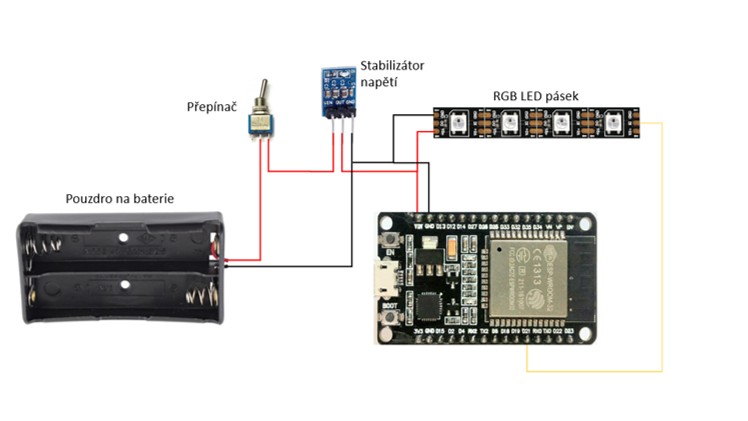
\includegraphics[width=1\textwidth]{img/01uvod/RGBSchema.png}
	\caption{Schéma zapojení obvodu}
	%	\label{fig:install-sdk-3}
\end{figure}

\subsection{ESP32-DevkitC}
\textit{ESP32-DevKitC} \cite{devkitc-datasheet} je výkonný programovatelný mikročip s WiFi a Bluetooth modulem, vyvinutý společností Espressif \cite{espressif}. Je kompatibilní s \textit{Arduinem} \cite{arduino}, se kterým se často využívá v~domácích hobby projektech. WiFi a Bluetooth modul dovoluje uživateli se na \textit{ESP32-DevKitC} připojit pomocí jakéhokoliv dálkového ovladače nebo mobilního telefonu a se zařízením manipulovat.
Součástí \textit{ESP32-DevKitC} desky je také micro-USB konektor, který dovoluje jak jednoduché nahrávání programu, tak jednoduché napájení. Pro další manipulaci a využití se~po obou stranách desky nachází vstupní a výstupní programovatelné piny, díky kterým lze k \textit{ESP32-DevKitC} připojit periferní zařízení, nebo zdroj napájení.

\begin{figure}[htbp]
	\centering
	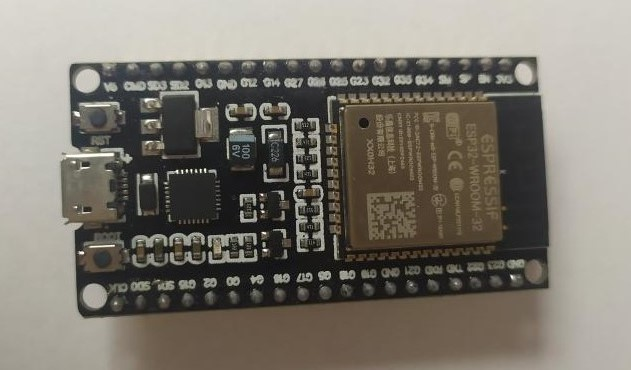
\includegraphics[width=0.5\textwidth]{img/02ele/ESPDevKit3.jpg}
	\caption{\textit{ESP32-DevKitC v4}}
	%	\label{fig:install-sdk-3}
\end{figure}

Při realizaci maturitní práce byly použity dvě verze desek: novější verze \textit{ESP32-DevKitC v4} a stejně výkonnou, ale vývojově o malinko starší verze \textit{ESP32-DevKitC v1}. Rozměry obou desek jsou 55~mm x 30~mm a liší se pouze pozicí a označením vstupních a výstupních pinů. Jinak je práce a manipulace s nimi stejná. 

\subsection{LED pásek WS2812}

Jedná se o programovatelný ohebný LED pásek, který se z důvodu nízké spotřeby a estetického vzhledu často využívá jako páskové osvětlení do interiérů a exteriérů. Pásek se~skládá z řady LED typu \textit{WS2812} \cite{WS2812}, které se pomocí kontroléru ve WS diodách dají jednoduše programovat. 

\begin{figure}[htbp]
	\centering
	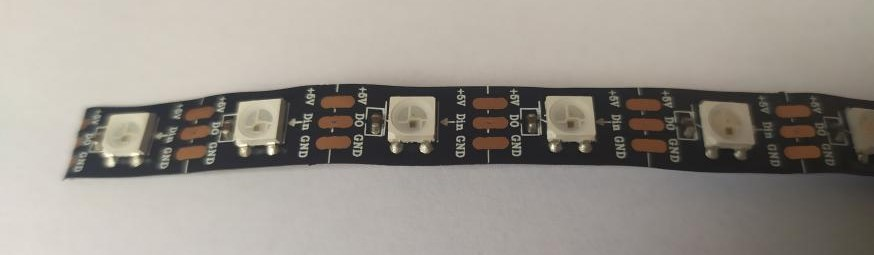
\includegraphics[width=0.5\textwidth]{img/02ele/OhebnyLedPasek2.jpg}
	%<<<<<<< Updated upstream
	\caption{Pásek \textit{WS2812}}
	%=======
	%	\caption{Pásek ws2812}
	%>>>>>>> Stashed changes
	%	\label{fig:install-sdk-3}
\end{figure}

Tento pásek se také často využívá jako výstupní modul pro \textit{Arduino}. Lze ho sehnat v~každém obchodě s elektronikou a elektrotechnickými součástkami, často pod marketingovým označením Neopixel  \cite{neopixel}. 

\subsection{DC Regulátor napětí 5,5 V}

% DollaTek 5,5V DC Voltage Regulator Step Down
Regulátor v obvodu slouží pro snížení vstupního napětí na napětí požadované. Tento DC~Regulátor napětí \cite{DollaTek} snižuje 5,8~V až 12~V na napětí 5~V. Sama deska \textit{ESP32-DevKitC} obsahuje vlastní stabilizátor, který opět snižuje napětí z 5~V na 3,3~V. Jmenovité napětí LED pásku je 5~V. Pokud by tedy bylo do obvodu puštěno vyšší napětí, mohlo by dojít jak ke zničení LED pásku, tak desky \textit{ESP32-DevKitC}.



    \begin{figure}[htbp]
	\centering
	\begin{minipage}[b]{0.5\textwidth}
		\centering
		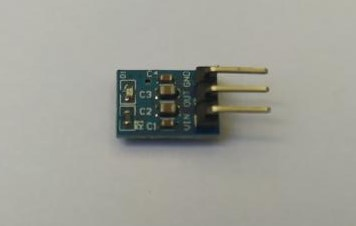
\includegraphics[width=0.75\textwidth]{img/02ele/Stepdownfront.jpg}
		\caption{Stabilizátor zepředu}
		%		\label{fig:gear-sketch1}
	\end{minipage}
	\hfill
	\begin{minipage}[b]{0.4\textwidth}
		\centering
		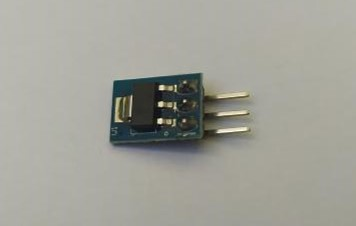
\includegraphics[width=1\textwidth]{img/02ele/Stepdownback.jpg}
		\caption{Stabilizátor zezadu}
		%		\label{fig:gear-sketch2}
	\end{minipage}
\end{figure}


\section{Možnosti napájení}

Důležitou součástí obvodu je také napájení, které by mělo mít dostatečně vysoké napětí, aby mohlo napájet obvod. Napájecí napětí obvodu musí být minimálně 5~V. Napadly mě tři možnosti řešení napájení \textit{ESP32-DevKitC} a LED pásku.


\subsection{4x AAA baterie 4,8 V}

Prvním nápadem bylo využít 4 tužkové AAA baterie s napájecím napětím 1,2~V, zapojené do série tak, aby jejich výsledné napětí bylo 4,8~V. Tato možnost se jevila velmi výhodně, protože vzhledem k nízkému napětí nebyl potřeba v obvodu regulátor napětí a sehnat AAA tužkové baterie je velmi jednoduché. Nevýhodou ale bylo, že by držák na 4 AAA tužkové baterie zabíral v základně hodně místa.
\newpage
Později se ale ukázalo, že není možné využít této možnosti, protože jmenovité napětí LED pásku bylo přesně 5,0~V, a i přesto, že ESP32-DevKitC fungoval bezchybně i na 4,8~V, LED pásek neměl dostatečně vysoké napětí, aby fungoval. Proto bylo potřeba zvážit jinou alternativu.


\subsection{Napájení Powerbankou}

Další možností bylo využít konektoru, který byl součástí desky  ESP32-DevKitC a přes něj napájet Powerbankou.

Výhoda tohoto napájení je, že v obvodu by nebyl potřeba stabilizátor. \textit{ESP32-DevKitC} je schopna si sama, pomocí svého regulátoru, snižovat převyšující napětí a napájet LED pásek pouze na 5V. Při realizaci této možnosti by nebylo potřeba řešit ani baterie, ani regulátor a celkově by se tato možnost vyplatila jako rychlé řešení problému. 

Co se týče umístění powerbanky. Byly zde opět dvě možnosti: %Nenapadlo mě jak jinak to formulovat
První možnost byla sehnat dostatečně malou powerbanku, aby se dala zabudovat do základny společně se zbytkem obvodu. 
%todo Je vážně správné slovo externí? 

Další možností bylo používat powerbanku jako externí zdroj, kdykoliv by bylo potřeba světla napájet. Oproti minulé možnosti by mohla mít powerbanka jakoukoliv velikost a tvar a~kdyby bylo potřeba, mohla by být nahrazena napájením z počítače nebo jakýkoliv kabelem.  

Stejně tak by nebyl problém s opakovatelným nabíjením Powerbanky.  V případě, že by Powerbanka byla zabudovaná vevnitř, stačilo by ji vytáhnout a znovu přes USB kabel nabít. 
V případě, že by Powerbanka sloužila jako externí zdroj, bylo by její znovunabíjení ještě jednodušší.
%(kdyby se powerbanka zabudovala dovnitř, základna by byla o mnoho větší než výsledná žárovka a kazilo by to estetický dojem, Dále jsem chtěla, aby byla světla autonomní, aby stačilo pouze zapnout tlačítko. Nelíbila se mi představa, že ze světla bude vést kabel až k powerbance.)


\subsection{Li-ion 18650}

Jako nejvhodnější možnost se mi ale jevilo využití dvou sériově zapojených Li-ion baterií 18650 \cite{liion} o napětí 3,6~V (dohromady 7,2~V), jejichž napětí se sice musí snižovat regulátorem napětí, ale zajišťují dostatečné napětí jak pro ESP tak pro LED. Rozměry baterií v držáku byly 75~mm x 42~mm x 20~mm.  Takže baterie byly dostatečně malé, aby se mohly uložit do základny se zbytkem obvodu. Li-ion baterie lze opakovaně nabíjet na speciální akumulátorové nabíječce, čímž se po delší době může výstupní napětí baterií malinko snížit, což ale v~našem případě nevadí, protože přebytek napětí na bateriích je dostatečně vysoký, abychom se nemuseli bát nedostačujícího napětí. 


\begin{figure}[htbp]
	\centering
	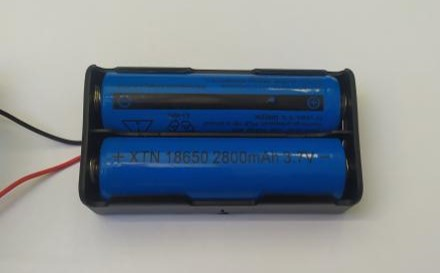
\includegraphics[width=0.45\textwidth]{img/02ele/Battery_Pack.jpg}
	\caption{Baterie}
	%	\label{fig:install-sdk-3}
\end{figure}



%Chtěla jsem aby zařízení bylo autonomní


\section{Nabíjení}
Nabíjení by v případě použití čtyř tužkových baterií AAA nebylo potřeba vůbec řešit, protože pokud by se baterie vybily, stačilo by jednoduše koupit nové. Stejně tak by nebyl moc velký problém při použití powerbanky, protože v případě vybití by stačilo powerbanku jednoduše znovu nabít.

S nabíjením Li-ion baterií to je ale trochu složitější. Ne každý doma vlastní speciální akumulátorovou nabíječku na Li-ion baterie, takže vyřešení nabíjení baterií je oproti dvěma předchozím možnostem napájení o malinko složitější. 
% Tato nabíječka ale není běžnou součástí každé domácnosti. 
Pro vyřešení této problematiky byla použita součástku \textit{TP4056} \cite{TP4056}.


\subsection*{Nabíječka Li-ion článku \textit{TP4056} micro-USB}
Jedná se o nabíjecí čip, určený pro nabíjení lithiových akumulátorů, který při připojení k~držáku na baterie dovoluje pomocí micro-USB konektoru dané baterie nabíjet. Modul nemá zkratovou ochranu, proto je při práci s ním potřeba opatrnost. Ochrana proti přepětí modulu je do 4,2~V, takže pro nás ideální. Dále jsou součástí modulu dvě indikační LED. Červená LED indikuje nabíjení. Modrá LED indikuje kompletní nabití. 

\begin{figure}[htbp]
	\centering
	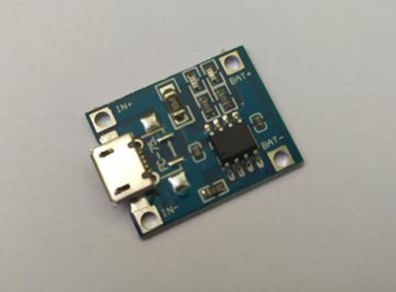
\includegraphics[width=0.3\textwidth]{img/02ele/Napajeciclanek.jpg}
	\caption{Nabíjecí článek}
	%	\label{fig:install-sdk-3}
\end{figure}

Nabíjení pomocí tohoto článku se dá opět vyřešit dvěma způsoby.

\begin{enumerate}
	\item Připojit nabíjecí modul přímo do obvodu
	\item Vytvořit vlastní nabíječku
\end{enumerate}


\subsection*{Připojení modulu do obvodu}
Jedna ze dvou možností byla připojit nabíjecí článek přímo do obvodu k bateriím, aby v~případě jejich vybití stačilo sundat vrchní díl základny a pomocí micro-USB konektoru na~modulu obě baterie znovu nabít.
Takhle metoda se mi zdála nevhodná z důvodu, že by základna po celou dobu nabíjení baterie musela být otevřena. 


\subsection*{Vlastní nabíječka}
%Vytvořit pomocí nabíjecího článku a držáku na baterky vlastní nabíječku
Druhá možnost se mi jevila podstatně přijatelnější. Plánem bylo vzít držák pro dvě baterie a na jeho vývody napájet 2 nabíjecí články. Na každou jednotlivou baterii se napájel článek zvlášť, protože článek neumí napájet baterie v sériovém zapojení.

Tato možnost se jevila jako vhodná a levná alternativa, jak vyřešit nabíjení baterií. 
%Problémem zůstává, že vyndávání Li-ion baterií, aby mohli být umístěny do nabíječky, bude celkem obtížné. V tu chvíli se ale tato možnost jevila mnohem jednodušeji, než znovu předělávat celý obvod.
%Bohužel jsem se spletla a zapájela to obráceně. No… Asi to nebylo tak jednoduché jak jsem psala. 

    \begin{figure}[htbp]
	\centering
	\begin{minipage}[b]{0.45\textwidth}
		\centering
		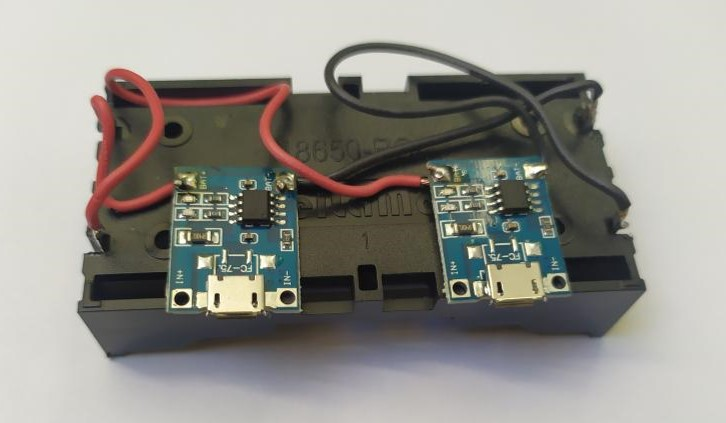
\includegraphics[width=1\textwidth]{img/02ele/Nabijecka.jpg}
		\caption{Nabíječka zepředu}
		%		\label{fig:gear-sketch1}
	\end{minipage}
	\qquad
	\begin{minipage}[b]{0.45\textwidth}
		\centering
		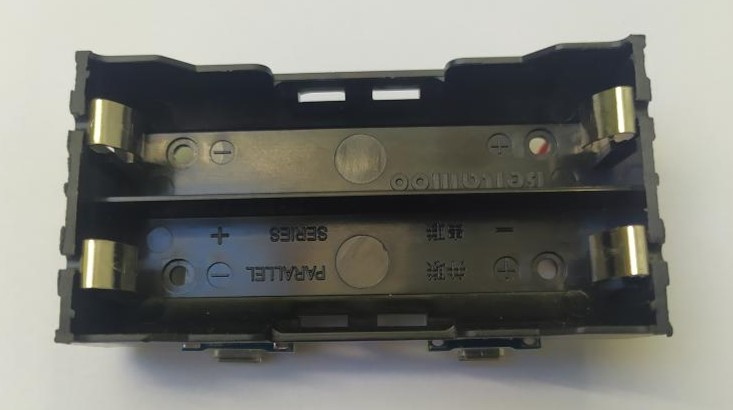
\includegraphics[width=1\textwidth]{img/02ele/Nabijecka2.jpg}
		\caption{Nabíječka zezadu}
		%		\label{fig:gear-sketch2}
	\end{minipage}
\end{figure}
\newpage





\chapter{Ovládání}
Ovládání LED světel je zajištěno pomocí WiFi modulu, jenž je součástí \textit{ESP32-DevKitC}. Plánem bylo připojit mobilní telefon na WiFi modul a využít ho jako dálkový ovladač. 

Toho bylo dosáhnuto za pomoci aplikace \textit{RBController} \cite{RBControler}, což je aplikace speciálně \textit{Robotárnou} \cite{robotarna} navržena na řízení a ovládání desek za pomoci WiFi Modulu. Na \textit{Robotárně} už několik let využívá pro dálkové řízení robotů pomocí mobilních telefonů. Tato aplikace byla také použita na Letním Robotickém táboře 2020 \cite{tabor}, který každoročně pořádá Dům Dětí a~Mládeže Helceletka \cite{helceletka}.

Prvním krokem bylo si ale v aplikaci vytvořit a umístit tlačítka na řídící plochu tam, kde jsem je chtěla mít. A přesně k tomu jsem využila webovou aplikaci \textit{Esp32-RBGridUI-Designer}, speciálně \textit{Robotárnou} navrženou pro tuto práci.


\section{Esp32-RBGridUI-Designer} 
\textit{Esp32-RBGridUI-Designer} \cite{designer} je webová aplikace, vytvořena \textit{Robotárnou} za účelem navrhnutí ovládacího panelu, který se zobrazí v aplikaci \textit{RBController}, při připojení uživatele k~WiFi modulu. 

Webová aplikace dovoluje uživateli určit počet, barvu a umístění tlačítek na ovládacím panelu. Aplikace má příjemné prostředí a dobře se s ní pracuje. 

Webová stránka {\em Esp32-RBGridUI-Designer} má rozložení: 


\begin{figure}[htbp]
	\centering
	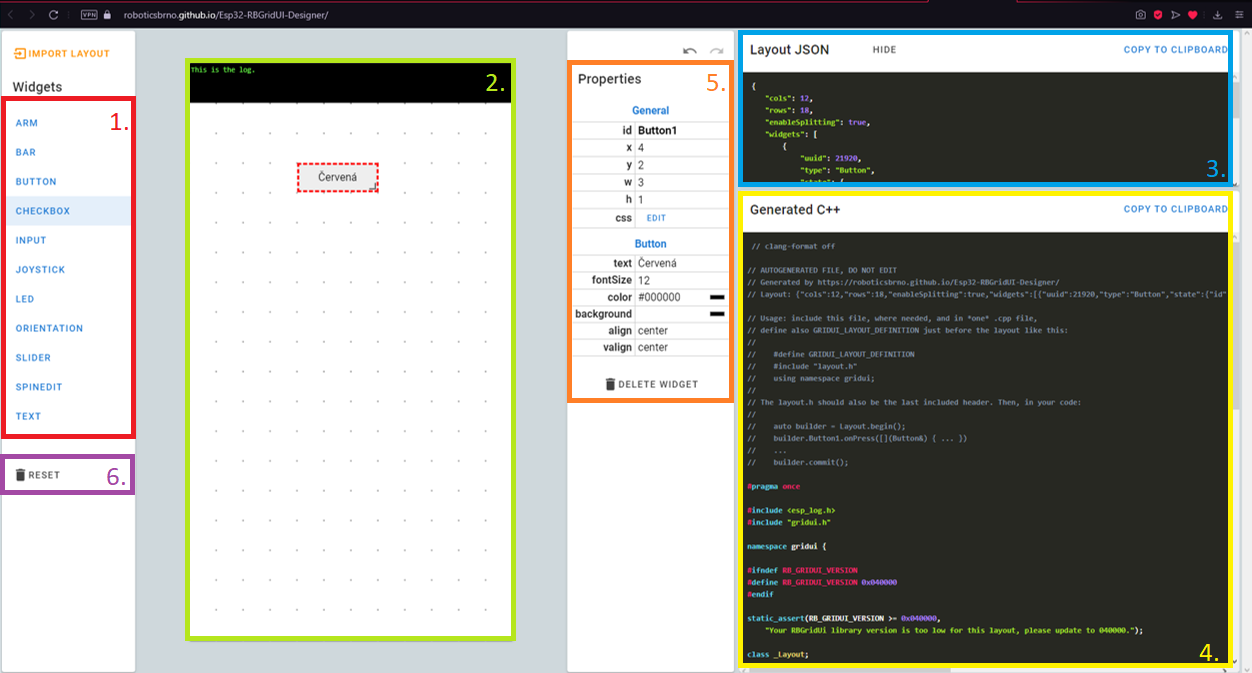
\includegraphics[width=1\textwidth]{img/03ovl/Esp32-RBGridUI-Designer.png}
	\caption{Prostředí stránky {\em Esp32-RBGridUI-Designer}}
	%	\label{fig:install-sdk-3}
\end{figure}

\begin{enumerate}
	\item Postranní lišta -- při kliknutí na jakoukoliv komponentu je uživatel schopen danou komponentu přetáhnout na manipulační plochu.
	\item Manipulační plocha, na kterou se umisťují komponenty z postranní lišty. Nastavuje se tu jejich poloha a umístění. Manipulační plocha určuje vzhled řídící plochy v aplikaci v mobilním telefonu při napojení na daný Wifi modul. 
	\item  Tuto tabulku pro práci s \textit{ESP32-DevKitC} potřebovat nebudeme.
	\item  Soubor Layout, který je potřeba stáhnout a nahrát do stejné složky, ve které máme hlavní program. Tento soubor nese informace o tom, jakým způsobem byly komponenty rozmístěny na manipulační polochu.
	\item Bližší specifikace, určující umístění, barvu a název tlačítka, které bylo vytvořeno na~manipulační ploše. Tyto informace je možné zde i měnit a upravovat. 
	\item Tlačítko Reset, které vymaže veškeré komponenty z manipulační plochy, a tím pádem i z Layoutu.
\end{enumerate}


% {\em Esp32-RBGridUI-Designer} je propojený s aplikací {\em RBControler,}  \cite{RBControler}

\section{Vytvoření tlačítek}
Plán byl vytvořit čtyři různá tlačítka, která by přepínala mezi čtyřmi různě barevnými módy světla. Tato tlačítka byla umístěna na ovládací plochu a přehledně pojmenována. 

Po vytvoření tlačítek v aplikaci bylo důležité uložit text, který se nacházel v kolonce \textit{Generated C++}. Stačilo daný text zkopírovat a vložit do textového souboru \textit{layout.txt} a~příponu \textit{.txt} přepsat na příponu \textit{.hpp}. Pak bylo potřeba uchovat tento soubor pro budoucí užití.
\newpage




\chapter{Program a jeho realizace}
Nejefektivnější se mi zdálo psát program v programovacím prostředí \textit{Visual Studio Code} \cite{Visualstudio}, se kterým jsem měla nejvíc zkušeností. 

Jedná se o bezplatný editor zdrojového kódu, vhodný pro programování v jakémkoliv programovacím jazyce, bez potřeby přepínání mezi editory. \textit{Visual Studio Code} má podporu programovacích jazyků jako jsou: Python, Java, C++, Javascript a mnoho dalších. 

Kromě \textit{Visual Studio Code} bylo při realizaci použito i jeho plug-in rozšíření s názvem \textit{PlatformIO} \cite{platformio}, což je soubor knihoven, kompatibilních s knihovnami od \textit{Robotárny}. \textit{Robotárna} toto rozšíření využívá a programuje v něm už léta.  Je skvěle kompatibilní s knihovnami \textit{Arduina} a~knihovnami \textit{SmartLeds}, které byly použity z důvodu jejich jednoduchosti a intuitivnosti při programování LED.
%Bylo použito vs. Požila jsem????



\section{Diagram programu }

\begin{figure}[htbp]
	\centering
	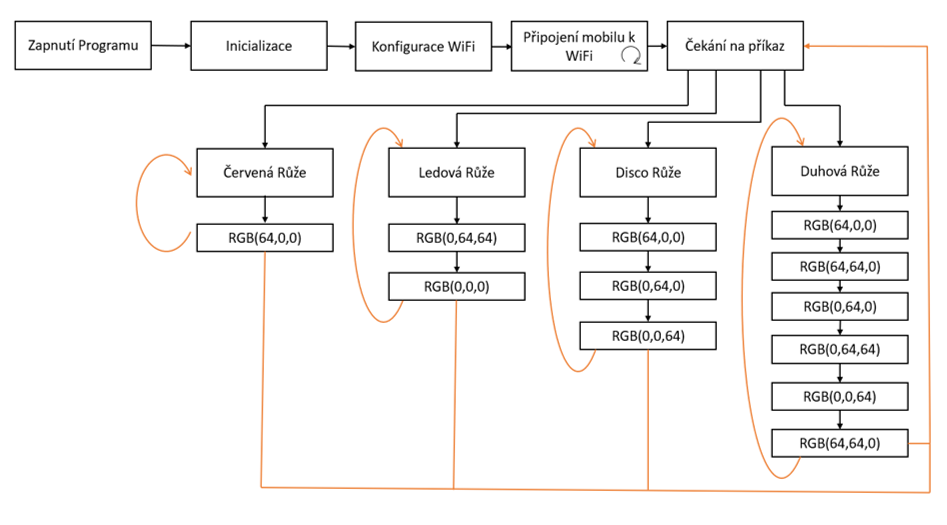
\includegraphics[width=1\textwidth]{img/04prog/Diagramprogramu.png}
	\caption{Blokový diagram programu}
	%	\label{fig:install-sdk-3}
\end{figure}

Tento blokový diagram ukazuje příkazy programu, jak jsou naprogramovány od spuštění (zmáčknutím tlačítka se začne provádět inicializace) až do vypnutí (proces vypnutí může být zahájen v~jakékoliv části programu, stačí jen sepnout tlačítko, a tím přerušit dodávku elektrické energie). 
\newpage

V dalších kapitolách jsou podrobněji rozepsané některé části programu.


\section{Inicializace}
V této části programu se začnou načítat a spouštět veškeré knihovny zahrnuté v programu. Mezi nimi je i soubor \textit{layout.hpp}, který byl vytvořen a uložen v předchozí kapitole. Jsou zde také informace, který je řídící pin LED pásku a kolik LED bude pásek obsahovat.


\section{Konfigurace WiFi a připojení mobilního telefonu k~Wifi}
%konfigurace = nastavení
V těchto částech programu se kompletně nastaví a zapne vysílaný WiFi signál. Nastaví se jméno a heslo, pod kterými se na WiFi lze připojit. V našem případě se jedná o WiFi s~názvem LEDLED a heslem „ledkyledky“. Dále se nastaví vlastník zařízení, název zařízení, čas kompilace zařízení a za pomoci souboru \textit{layout.hpp} sa nastaví podoba ovládacího panelu v mobilním telefonu. 

Po připojení mobilního telefonu na WiFi a zobrazení ovládacího panelu v aplikaci \textit{RBController} už program v \textit{ESP32-DevKitC} jenom čeká na jeden z naprogramovaných příkazů, aby ho mohl provést.
%Inicializace zařízení? 


\section{Příkazy}
Příkazy se v tomhle případě rozumí naše 4 nadefinovaná tlačítka, které jsme si vytvořili v~předchozí kapitole. Každé z těchto tlačítek má v programu přidělenou vlastní funkci, kterou po zmáčknutí provede.

Barva světel je naprogramovaná pomocí RGB spektra. V některých případech se jedná o~jednu prostou barvu, v jiných o donekonečna se opakující se různobarevný cyklus. 

Tlačítka a jejich příkazy: 
\begin{itemize}
	\item \textbf{Červená růže} – barva LED se nastaví na RGB(64,0,0) – tedy červenou barvu. Touto barvou zařízení září po celou dobu. 
	
	\item \textbf{Ledová růže} – jedná se o cyklický barevný přechod. Světle modré světlo se pomalu rozsvěcuje a poté zhasíná, čímž vytváří pulzující dojem magického předmětu. 
	
	\item \textbf{Disko růže} – cyklus, ve kterém se zběsile střídají 3 barvy (červená, modrá a zelená). Bylo původně spíše myšleno jako recese a nachází se zde pro zastoupení různorodosti barevných kombinací. 
	
	\item \textbf{Duhová růže} – mnohobarevný cyklus, který projde celým barevným spektrem. 
\end{itemize}


Veškeré příkazy jsou provedeny pomocí nadefinované funkce \textit{SetLedAll}, která při zadání tří čísel automaticky veškeré LED na pásku nastaví danou RGB barvu a není potřeba každou jednotlivou LED nastavovat samostatně. 

Při programovaní LED pásku nebyla použita maximální intenzita LED pásku. Rozsah RGB je sice od 0 do 255, ale při použití plné intenzity 255 bylo světlo z LED až moc jasné a po delší práci a koukání se na barvy z něj mě začaly bolet oči a hlava. Proto byla světelná intenzita LED pásku snížena na čtvrtinu. 
\newpage

\chapter{Výroba růže}
Původním záměrem bylo vytvořit svítící lampičku ve tvaru růže. Vzorem pro výrobu růže byl plastový uzávěr od lahvičky s vůní ve tvaru růže, s rozměry: přibližně 6~cm široký a 3~cm vysoký. Tato růže byla použita na výrobu formy. Forma byla později opakovaně použita na výrobu tří téměř identických odlitků.
%Mohla jsem se domluvit s umělcem, aby růže byla ze skla, mohla jsem ji vytisknout na 3D tiskárně. Já jsem se ji ale rozhodla odlít, protože mě zaujala práce s křišťálovou pryskyřicí. 

%*Obrázek k vzoru*


\section{Silikonová forma}

Rozhodla jsem se že formu vyrobím z odlévacího silikonu. Odlévací silikony mají skvělé kopírovací vlastnosti a mají i dostatečnou pružnost, potřebnou k dobrému odformování komplikovaných výrobků. Pokud je forma dobře udělaná, lze ji používat opakovaně.



\begin{figure}[htbp]
	\centering
%	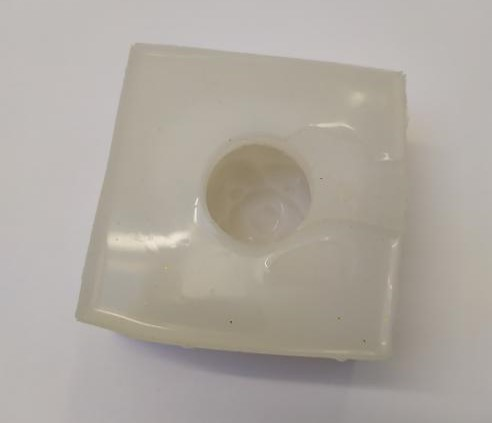
\includegraphics[width=1\textwidth]{img/05odl/Siliconemold.jpg}
%	\caption{Silikonová forma}
	%	\label{fig:install-sdk-3}
\end{figure}
 

%\subsection{Leukopren žlutý silikon}

\subsection*{Adiční silikon GMS A30 (Silikon)}

%Druhým druhem silikonu byl Adiční silikon GMS A30.
Na výrobu formy jsem použila \textit{Adiční silikon GMS A30}  \cite{silikon} z internetového obchodu \textit{Levnetmely.cz}  \cite{tmely}. Jedná se o dvousložkový, dobře tekutý silikon s velmi dobrou kopírovací schopností, schopný zkopírovat jak povrch obyčejného papíru, tak dřeva s letokruhy.

Tento silikon se používá na výrobu forem, například pro odlévání epoxidové pryskyřice, sádry nebo vosku. Dále se využívá na výrobu těsnění nebo zalévání součástek v elektroprůmyslu.


\subsection*{Práce se silikonem}
Balení \textit{Adičního silikonu GMS A30} se skládá ze dvou složek: složky~A a složky~B. Tyto dvě složky se musí smíchat v hmotnostním poměru 1:1. Při míchání je potřeba dát pozor, aby se do silikonu nedostaly bublinky, které by mohly znehodnotit formu a zdeformovat kopírovaný tvar.

V případě použití kompresoru by stačilo veškerý vzduch odsát, a tím způsobem se zbavit bublinek. Protože ale kompresor nevlastním, malému množství bublinek jsem se nevyhnula. Při práci se silikonem je potřeba dbát na bezpečnost práce a při manipulaci se silikonem mít na sobě ochranné brýle a rukavice.

%*Obrázek formy*

Po přibližně 24 hodinách bývá výsledkem středně tvrdá, odolná silikonová pryžová forma, se skvělým odformováním. V našem případě ale odformování problematizoval komplikovaný tvar květiny.


\begin{figure}[htbp]
	\centering
	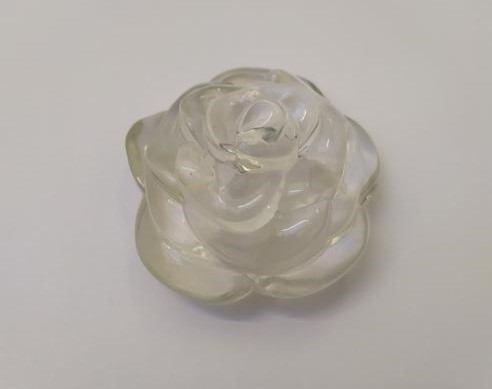
\includegraphics[width=0.5
	\textwidth]{img/05odl/Rose.jpg}
	\caption{Odlitá růže}
	%	\label{fig:install-sdk-3}
\end{figure}

\section{Pryskyřice}
Křišťálová pryskyřice  \cite{pryskyrice} (Epoxy Resin) je dvousložková průhledná odlévací směs často používaná na výrobu bižuterie, různých dekorací nebo glazování povrchů. Dobře se s ní pracuje, její zápach je nízký, a po vytvrdnutí je její povrch lesklý a nesmršťuje se. 

Pro realizaci tohoto projektu byla pryskyřice vybrána z důvodu dobré imitace skla a~zároveň nízké křehkosti tohoto materiálu. 
%Tato pryskyřice byla vybrána i z důvodu, že dobře imituje sklo, ale zase postrádá jeho křehkost.
Při odlévání růže byla konkrétně použita křišťálová pryskyřice od firmy \textit{Pebeo}  \cite{pebeo}, sehnatelná v jakémkoliv specializovaném uměleckém obchodě nebo obchodě pro kutily. 


\subsection*{Práce s pryskyřicí}

Pro použití pryskyřice je třeba smíchat složku A a složku B. Tyto dvě složky se  smíchají v~hmotnostním poměru 2:1. Při odvažování je důležitá přesnost. Dále je duležité obě složky dobře promíchat, jinak by mohlo dojít ke špatnému vytvrzení výrobku. Při míchání je třeba dávat pozor, aby se do pryskyřice nedostaly bublinky. Poté se daná směs vylije do předem připravené formy nebo na povrch, který chceme glazovat. Pryskyřici trvá 24 až 48 hodin, než zatvrdne. Křišťálová pryskyřice je chemikálie a proto se, z důvodů možných alergických reakcí a podráždění dýchacích cest, doporučuje při manipulaci s pryskyřicí nosit ochranné brýle, rukavice a respirátor. 

Před vylitím pryskyřice do předem připravené formy je prý vhodné danou formu vytřít speciální vazelínou, která prodlužuje životnost formy a která brání jejímu poškození při vyjímání odlitku. Tento způsob se ale v našem případě, při odlévání pryskyřičné růže, neosvědčil. Vazelína se smíchala s odlévací pryskyřicí a ve výrobku se vytvořil bílý mléčný kal, který znehodnotil výrobek a pokazil sklovitý dojem pryskyřice.









\chapter{Základna}
%Základna Jako poslední část jsem potřebovala krabičku – nějakou základnu, která by sjednotila jednotlivé komponenty do jednoho kompletního celku. 
Jako poslední už mi zbývalo jen udělat základnu, nebo také krabičku, do které bych mohla schovat elektrický obvod, a na její víko umístit růži.
Rozměry krabičky byly designované podle nejrozměrnější komponenty v elektrickém obvodu, jednalo se o držák s bateriemi, jehož rozměry jsou 75~mm x 42~mm x 20~mm. Druhou největší komponenta byla deska \textit{ESP32-DevKitC} s rozměry: 55m~m x 30~mm s~výškou 10~mm.
Podle výše zmíněných dvou nevětších komponent byly stanoveny přibližné vnitřní rozměry základny: 82~mm x 82~mm x 45~mm, které zaručovaly, že se do základny vejde jak \textit{ESP32-DevKitC} tak baterie, zůstane nějaká rezerva na kabely a další komponenty a základna nebude o moc větší než růže.  
Aby byla ověřena správnost rozměrů, byl podle nich vytvořen první prototyp.
%abych ověřila správnost rozměrů, rozhodla jsem se podle nich vytvořit první prototyp.
%82 mm x 82 mm x 45 mm,



\section{První prototyp}
První prototyp byl vyroben ručně ze 4~mm široké překližky. Podle toho se poté přibližně odvodily vnější rozměry základny. U tohoto prototypu to přibližně bylo: 90 x 90 x 50~mm. Tato práce nebyla profesionální, proto se výsledné rozměry základny nepatrně lišily (+/-2~mm).
%jsem vyrobila ručně

Pro výrobu prototypu bylo z překližky vyřezáno šest dílů: Vrchní a spodní díl 90~mm x 90~mm a čtyři boční stěny o rozměrech 45 x 90~mm a 45 x 82~mm. Do vrchního dílu byl vyřezán kruhový otvor o průměru 28~mm, pro umístění odlité růže a do jednoho bočního dílu byl vyvrtán vrtačkou otvor pro menší přepínací tlačítko. Do rohů byly přilepeny lepidlem \textit{Herkules} špalíčky 10~x~10~mm, které držely všechny desky základny u sebe a později sloužily pro držení vrchního dílu a růží pomocí šroubků. Takže se vrchní díl s růží mohl kdykoliv sundat a bylo možné manipulovat s elektrotechnikou uvnitř.

%todo jak je to s přívlastky? 
%Dva čtverce o šířce přibližně 90 mm
%2 obdélníky o výšce 45 mm a délce 90
%2 obdélníky o výšce 45 mm a délce 82
\begin{figure}[htbp]
	\centering
	\begin{minipage}[b]{0.5\textwidth}
		\centering
		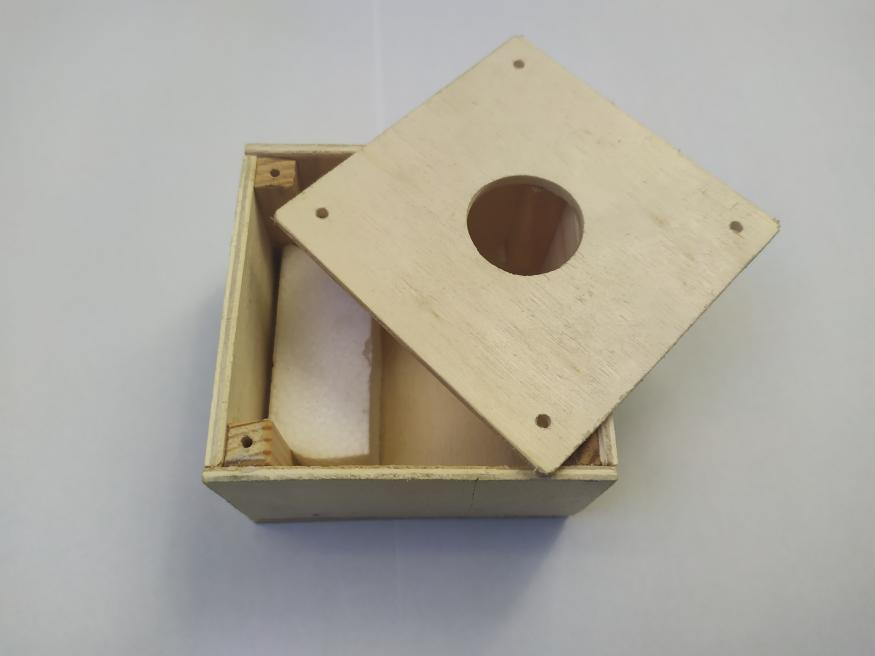
\includegraphics[width=0.8\textwidth]{img/06zakl/Amazakladna.jpg}
		\caption{První prototyp}
		%		\label{fig:gear-sketch1}
	\end{minipage}
	\qquad
	\begin{minipage}[b]{0.4\textwidth}
		\centering
		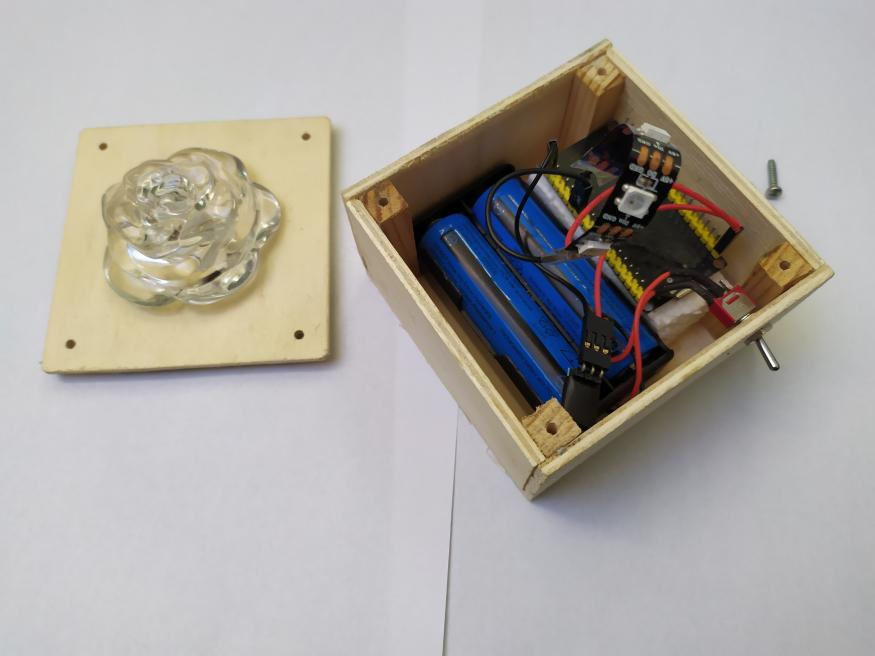
\includegraphics[width=1\textwidth]{img/06zakl/1prototypele.jpg}
		\caption{Kompletní  prototyp}
		%		\label{fig:gear-sketch2}
	\end{minipage}
\end{figure}

Po sestavení krabičky byl pro kontrolu do krabičky vložen náš elektrický obvod.
Jelikož pokus s prvním prototypem proběhl úspěšně, začala jsem pracovat na dokonalejším druhém prototypu.


\section{Druhý prototyp }
Druhý prototyp základny byl také vyroben ze dřeva, tentokrát ale byly jednotlivé stěny krabičky vypáleny na laseru. Díky čemuž prototyp působil profesionálněji. Při této výrobě byla použita překližky o síle 3~mm. Jednotlivé díly krabičky byly navrženy v~programu \textit{MakerCaser} \cite{makercase}, který po zadání vnitřních rozměrů a tloušťky překližky vygeneroval výkres hotové krabičky i s hotovými okrajovými zámky, aby se do rohů prototypu tentokrát nemusely lepit špalíčky. 

\subsection*{Práce s Lightburnem}
\textit{Lightburn} \cite{lightburn} je placený editační software, který škola používá pro práci s laserovými řezačkami. 
Stačilo do tohoto programu pouze nahrát uložený soubor ze stránky \textit{MakerCaser}, přidat otvor ve vrchním dílu a logo školy. Poté stačilo upravený soubor nahrát ve formátu \textit{.svg} do školní laserové tiskárny a krabičku vypálit. Výsledek působil reprezentativně, takže se nakonec na laseru vypálily i krabičky pro zbývající výrobky. 
 %Jinak zbytek ostatní  zůstal beze změny.


%todo *Obrázek*

\begin{figure}[htbp]
	\centering
	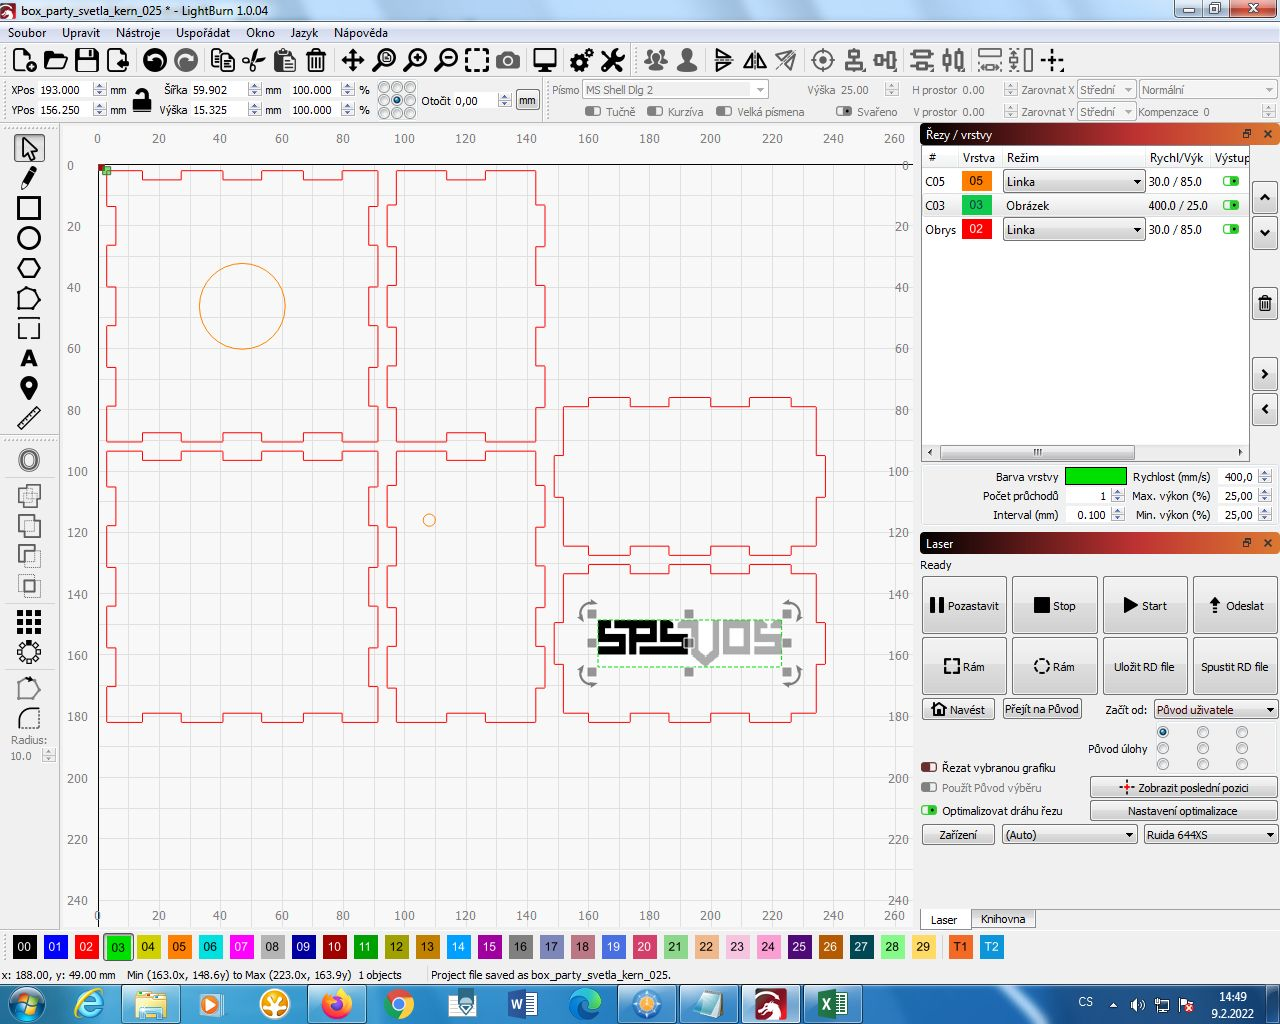
\includegraphics[width=0.5\textwidth]{img/06zakl/LightBurn_ukazka.jpg}
	\caption{Prostředí LightBurn}
	%	\label{fig:install-sdk-3}
\end{figure}

\subsection*{Vložení elektrotechniky a růže do krabičky}
Krabičky pak byly složeny do své finální podoby a jejich rohy byly zpevněny lepidlem \textit{Herkules}, aby krabičky lépe držely pohromadě. Jediný kus, který nebyl přilepen, byl vrchní díl s růží, aby se kdykoliv v případě potřeby mohl sundat. 


Poté byl vložen elektrický obvod. Přepínač byl upevněn do otvoru na tlačítko, do základny byl položen opatrně držák s bateriemi a \textit{ESP32-DevKitC} byl umístěn na kousek polystyrenu, aby v krabičce jen tak neležel a nepohyboval se. 
%Todo lépe zdůvodnit ten polystyren, kabely byli douhé. (nevhodně ustřižené)
Ohebný LED pásek byl opatrně ohnut do obloučku a vložen do otvoru v růži. Poté bylo opatrně přiděláno vrchní víko a bylo hotovo. 
%todo nevím jak to zakončit. 

%\enlargethispage{1}

\begin{figure}[htbp]
	\centering
	\begin{minipage}[b]{0.45\textwidth}
		\centering
		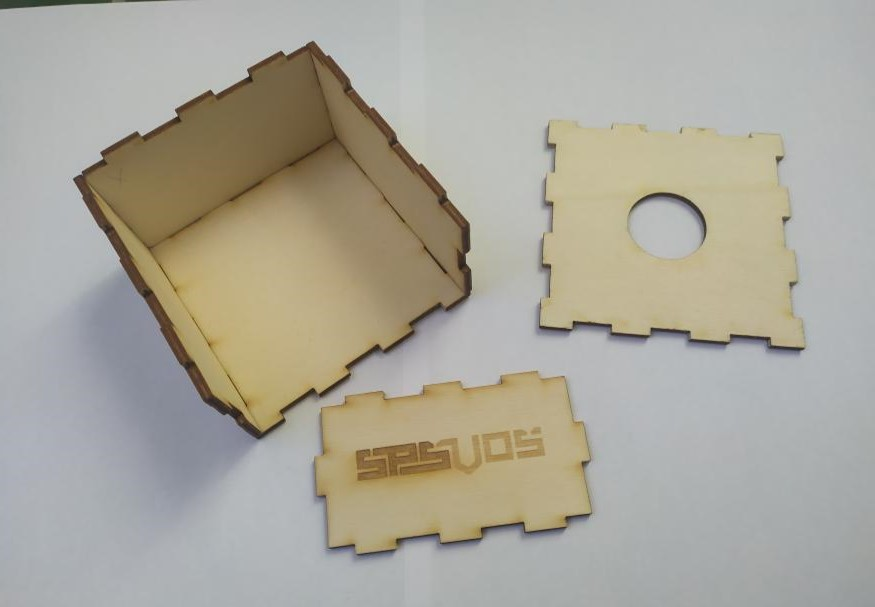
\includegraphics[width=1.1\textwidth]{img/06zakl/Box.jpg}
		\caption{2. prototyp}
		%		\label{fig:gear-sketch1}
	\end{minipage}
	\qquad
	\begin{minipage}[b]{0.45\textwidth}
		\centering
		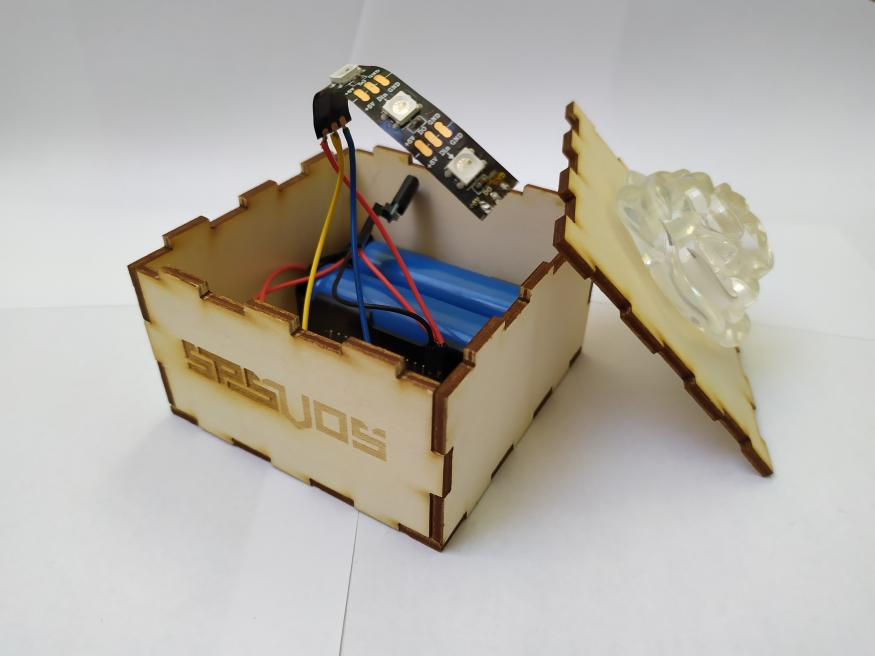
\includegraphics[width=1.01\textwidth]{img/06zakl/2prototypele2.jpg}
		\caption{2. prototyp s elektronikou}
		%		\label{fig:gear-sketch2}
	\end{minipage}
\end{figure}


\newpage


\chapter{Závěr}
Cílem mé dlouhodobé maturitní práce bylo  navrhnout a vyrobit svítící dekoraci pro vnitřní použití 
v počtu
alespoň tří kusů, která bude dálkově ovladatelná, bude umožňovat
měnit barvy světla
a bude pěkně vypadat.

Nejdříve jsem sestavila obvod, který řídí desku ESP32-DevkitC. Tento obvod se zapíná a~vypíná jediným přepínačem, který přerušuje a spojuje obvod. Součástí obvodu je kromě li-ion baterií také regulátor napětí, které napětí baterií sráží na požadovanou hodnotu. Dodatečně jsem k bateriím vytvořila ještě nabíječku, kterou se kdykoliv baterie mohly znovu nabít. 

Navrhla jsem si v aplikaci ovládací panel s tlačítky a naprogramovala ESP32-DevkitC tak, aby se pomocí jeho WiFi modulu daly jednotlivé módy světla z mobilního zařízení bezdrátově ovládat.  

Dále jsem si vytvořila silikonovou formu, do které jsem opakovaně odlila z křišťálové pryskyřice 3 růže, abych je mohla později použít jako žárovky na jednotlivé výrobky. 

Jako poslední jsem navrhla základnu, do které jsem vložila elektrický obvod, k vrchnímu dílu jsem připojila růži, která sloužila jako lampička a skrz kterou LED pásek prosvěcoval do prostoru. 

Vyrobila jsem celkem tři kusy dekorací. Všechna tato zařízení fungují podle očekávání a~splňují parametry zadání. 

Zdrojové soubory a texty k této dlouhodobé maturitní práci jsou umístěny také na mém github účtu \cite{github}.





%Prototyp světla je ke dni odevzdání ročníkové práce plně funkční. Do budoucna by se dal zkonstruovat obal, ve kterém by byla uložená elektronika (hlavně ESP32-DevKitC) a průhledný tvar, skrz který by LED zářily. Dále by se dalo vyrobit a zprovoznit těchto světel víc a zařídit, aby každé z nich bylo propojeno přes wifi s mobilním telefonem.


%Tato ročníková práce mi dala hodně zabrat. Ne proto, že bych měla složité téma a nebo program by byl složitý na naprogramování, ale problém byl v tom, že jsem se musela často učit pracovat s programy a věcmi, se kterými jsem předtím nepracovala. Naučila jsem se pracovat s ESP32 a inteligentními LED světly, naučila jsem se je programovat a dokonce se napojit na ESP32-DevkitC mobilním telefonem a pomocí něj ESP32-DevkitC ovládat.
%Celkově mě ale práce na této ročníkové práci bavila a dala mi do budoucna spoustu zkušeností, které se jistě budou hodit. 

 



\clearpage
\phantomsection

%\appendix
%\addcontentsline{toc}{chapter}{Přílohy}

% Prilohy
%\input{CHAPTERS/100 - PRILOHY.tex}

\input literatura.tex


\listoffigures
\addcontentsline{toc}{chapter}{Seznam obrázků}

\newpage

\chapter*{Obrazová příloha}

\begin{figure}[htbp]
	\centering
	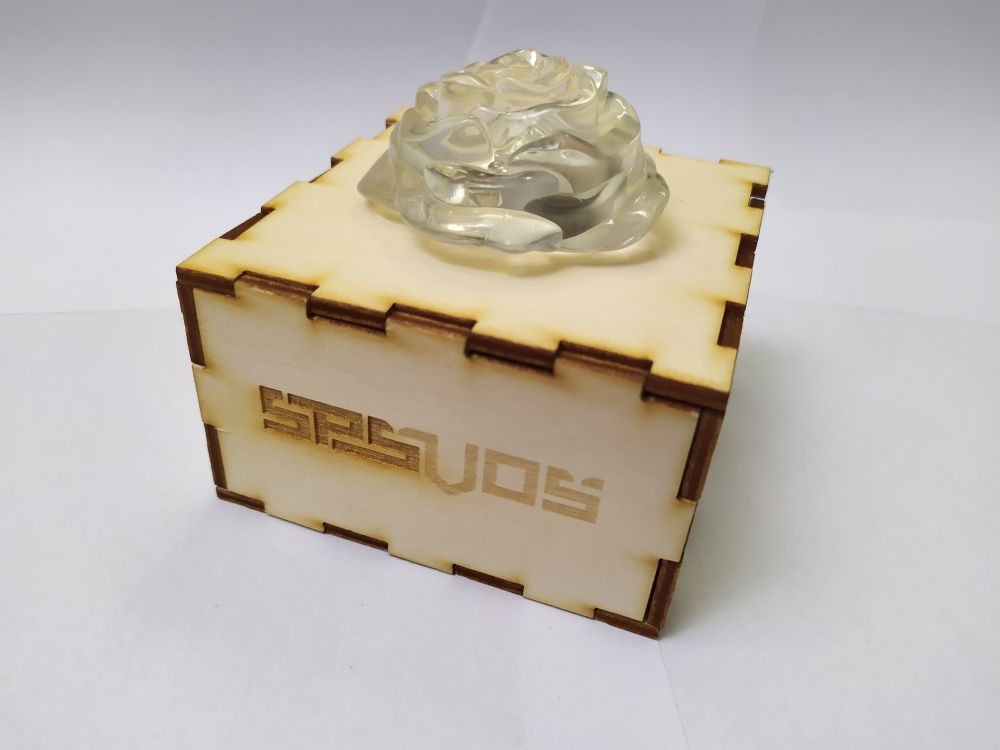
\includegraphics[width=1.0
	\textwidth]{img/06zakl/hotovo.jpg}
	\caption{Hotový výrobek}
	%	\label{fig:install-sdk-3}
\end{figure}

%\listoftables
%\addcontentsline{toc}{chapter}{Seznam tabulek}

\end{document}

%todo příloha program 
